\documentclass[11pt,a4paper]{article}

\usepackage[utf8]{inputenc}
\usepackage[T1]{fontenc}
\usepackage[spanish,es-noshorthands,es-tabla,es-nodecimaldot]{babel}
\usepackage[margin=2cm]{geometry}
\usepackage{amsmath,amssymb}
\usepackage{graphicx}
\usepackage{booktabs}
\usepackage{array}
\usepackage{xcolor}
\usepackage{enumitem}
\usepackage{listings}
\usepackage[section]{placeins}
\usepackage[hidelinks]{hyperref}
\usepackage[ruled,vlined,linesnumbered]{algorithm2e}

% Estilo del pseudocodigo (como en las diapositivas del curso)
\SetKwInput{KwEntrada}{Entrada}
\SetKwInput{KwSalida}{Salida}
\SetKwFor{ParaPar}{for}{\textcolor{red}{\textbf{pardo}}}{}
\newcommand{\comentario}[1]{\ttfamily #1}
\SetCommentSty{comentario}
\SetKwComment{tcp}{// }{}
\DontPrintSemicolon
\SetAlgorithmName{Algorithm}{Algorithm}{Lista de algoritmos}

\lstset{language=Python, basicstyle=\ttfamily\footnotesize, keywordstyle=\color{blue!60!black}\bfseries,
  commentstyle=\color{gray}, frame=lines, numbers=left, numberstyle=\tiny\color{gray}, columns=fullflexible,
  showstringspaces=false, breaklines=true}
\renewcommand{\lstlistingname}{Listado}

\newcommand{\ntr}{n_{tr}}
\newcommand{\nte}{n_{te}}

\setlength{\parskip}{3pt}
\setlength{\emergencystretch}{2em}

\begin{document}

\begin{center}
{\large \textbf{CS4052 Computación Paralela y Distribuida} -- 2026-II}\\[2pt]
Proyecto de Laboratorio -- \textbf{Entrega final}\\[10pt]
{\LARGE \textbf{Caso 5: KNN en paralelo con MPI (mpi4py)}}\\[4pt]
{\large Clasificación de dígitos (\textit{load\_digits})}\\[10pt]
Profesor: José Fiestas \quad -- \quad Grupo 7
\end{center}

\begin{table}[h]
\centering
\begin{tabular}{lc}
\toprule
\textbf{Integrante} & \textbf{Participación} \\
\midrule
Barzola Estrella, Johar Jared & 100\,\% \\
Huaman Casma, Leonardo Fabian & 100\,\% \\
Izaguirre Zavaleta, Luis Fernando & 100\,\% \\
\bottomrule
\end{tabular}
\\[3pt]
{\small (100\,\% indica que el integrante contribuyó en forma equitativa al resto)}
\end{table}

%====================================================================
\section{Introducción}

KNN (\textit{k-nearest neighbors}) es un algoritmo de clasificación supervisada: para clasificar un punto nuevo calcula su distancia a todos los puntos de entrenamiento, toma los $k$ más cercanos y le asigna la etiqueta que más se repite entre ellos. En este proyecto paralelizamos con mpi4py [3] el código secuencial \texttt{knn\_digits\_sec.py} [2], que clasifica las imágenes de dígitos de \textit{load\_digits} [4]: 1797 imágenes de $8\times 8$ píxeles ($d = 64$), divididas en $\ntr = 1437$ de entrenamiento y $\nte = 360$ de prueba, con $k = 3$. El código base da una precisión (\textit{accuracy}) de 0,9833.

El trabajo más costoso es calcular las $\ntr\cdot\nte = 517\,320$ distancias, que son independientes entre sí. Siguiendo el DAG del enunciado [1] (Figura~\ref{fig:dag}), el proceso 0 (maestro) envía la data de prueba a todos (\texttt{comm.bcast}), reparte la data de entrenamiento en bloques de $\ntr/p$ (\texttt{comm.scatter}), cada proceso calcula sus $k$ vecinos locales para cada punto de prueba y el maestro los recolecta (\texttt{comm.gather}), elige los $k$ más cercanos de todos y vota.

\begin{figure}[!htb]
\centering
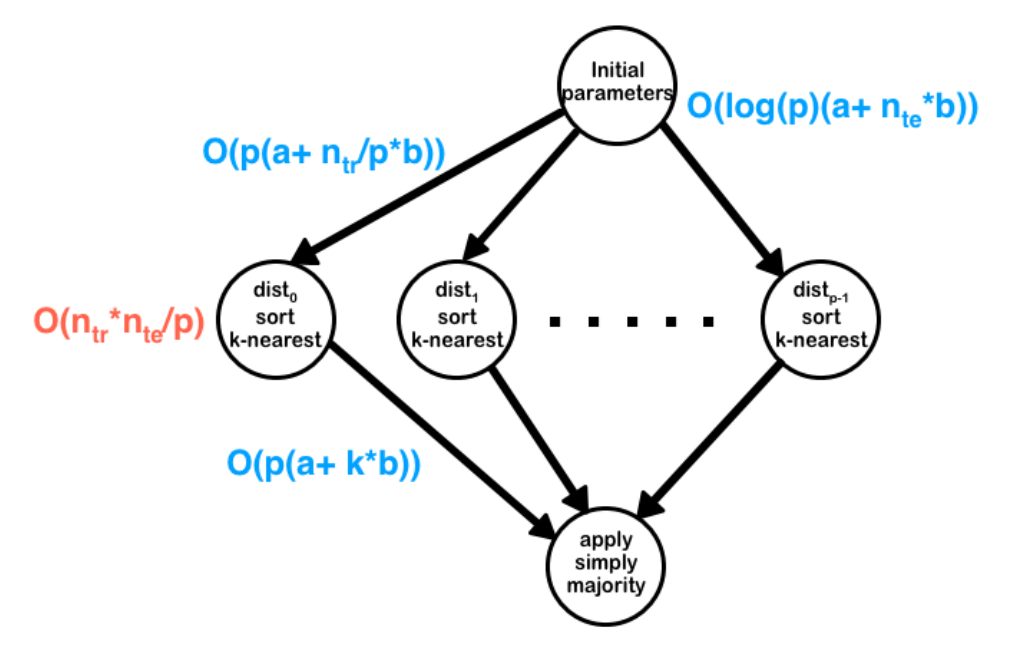
\includegraphics[width=0.46\textwidth]{dag_knn.png}
\caption{DAG del KNN en paralelo. En azul, los costos de comunicación; en rojo, el costo de cómputo de cada proceso. Los costos de scatter y gather corresponden a una topología lineal; MPI usa árboles (Sección~\ref{sec:dag}). Fuente: enunciado del proyecto [1].}
\label{fig:dag}
\end{figure}

En la entrega parcial presentamos el PRAM y las métricas. Para esta entrega final escribimos el código en tres versiones beta y una mejora con reducción en árbol, las validamos contra el código secuencial, medimos los tiempos de ejecución, cómputo y comunicación para $p \in \{1,2,4,6,8\}$ y cuatro tamaños del problema (de $n = 449$ a $n = 28\,752$), normalizamos la expresión teórica para compararla con las mediciones y analizamos el \textit{speedup}, los FLOP/s y la escalabilidad. Los resultados principales son:
\begin{itemize}[nosep]
  \item Las tres versiones y la mejora con reducción dan exactamente las mismas predicciones que el código base para $p = 1$ a $8$ (precisión 0,9833).
  \item La versión final (beta 3) es 38 veces más rápida que el código base en un solo proceso, y con $p = 8$ llega a $S = 7{,}2$ con $n = 1797$ y $S = 9{,}2$ con $n = 28\,752$.
  \item El modelo teórico normalizado reproduce los tiempos medidos con $R^2 = 0{,}998$ y un error relativo medio de 8\,\%.
  \item La cantidad óptima de procesos crece con el tamaño del problema: $p_{opt} \approx 7$ para $n = 449$ y $p_{opt} \approx 18$ para $n = 1797$.
  \item El algoritmo escala si $n = \Theta(k\,p^2)$ (isoeficiencia); los resultados con $p \le 8$ son consistentes con esa condición.
  \item La reducción en árbol (\texttt{comm.reduce}) acorta los pasos 5 a 7 hasta un 33\,\% con $p = 8$, pero el tiempo total casi no cambia: el ahorro es pequeño.
\end{itemize}

%====================================================================
\section{Método}

\subsection{Algoritmo secuencial y tamaño del problema}
\label{sec:secuencial}

Llamamos $n$ al número total de imágenes. El código base divide los datos en 80/20, así que $\ntr = 0{,}8\,n$ y $\nte = 0{,}2\,n$: basta un solo $n$ para describir el problema, y las dos partes crecen juntas.

Por cada punto de prueba, el código base calcula $\ntr$ distancias euclidianas de $O(d)$ operaciones, las ordena con \texttt{np.argsort} ($O(\ntr\log\ntr)$) y vota entre los $k$ vecinos con \texttt{Counter} ($O(k)$). Entonces
\[
T_s(n) = O\big(\nte\,(\ntr\, d + \ntr \log \ntr + k)\big) = O(n^2 \log n),
\]
porque $d$ y $k$ son constantes. Con los tamaños que usamos, $d = 64 > \log_2 \ntr$ ($\approx 10{,}5$ con los datos originales y a lo más 16,5), así que esperábamos que el cálculo de distancias, $O(\ntr\,\nte\,d) = O(n^2)$, pesara más que el ordenamiento. Ese es el costo de cómputo del DAG, $O(\ntr\cdot\nte)$, y también el del mejor algoritmo secuencial, que elige los $k$ menores sin ordenar todo (por ejemplo, con \texttt{np.argpartition}). (En la Sección~\ref{sec:norma} vemos que en la beta 3 el término del ordenamiento pesa más de lo que supusimos.)

\subsection{Diseño con el método de Foster}
\label{sec:foster}

Seguimos los cuatro pasos del método de Foster tal como los ve el curso (U1.2 y la PD01 [5], [6]).

\textbf{Particionamiento.} Usamos descomposición del dominio sobre la data de mayor tamaño, la de entrenamiento. La tarea primitiva es la distancia entre un punto de prueba y uno de entrenamiento: $\ntr\cdot\nte = 517\,320$ tareas con los datos originales, todas de costo $O(d)$ y muchas más que procesos (Figura~\ref{fig:foster}).

\textbf{Comunicación.} Cada tarea necesita sus dos puntos y entrega su distancia a la selección de los $k$ vecinos de su punto de prueba: las tareas de una misma fila se combinan en una reducción, con del orden de $\ntr\cdot\nte$ canales. Esta comunicación es \textit{overhead}: no existe en el algoritmo secuencial.

\textbf{Aglomeración.} Agrupamos en una sola tarea todas las distancias de un bloque de $\ntr/p$ puntos de entrenamiento contra los $\nte$ puntos de prueba, y hacemos que cada bloque devuelva solo sus $k$ mejores candidatos por punto de prueba en lugar de todas sus distancias. Así quedan del orden de $3p$ canales: un broadcast, un scatter y un gather por bloque. Elegir solo $k$ candidatos por bloque no cambia el resultado: si un punto es uno de los $k$ vecinos más cercanos entre todos los datos de entrenamiento, también lo es dentro de su bloque (si no, el bloque tendría $k$ puntos más cercanos y el punto no podría ser vecino global). \textbf{Esta aglomeración es la que convierte el PRAM ideal de la Sección~\ref{sec:pram} en el algoritmo distribuido del DAG} (Sección~\ref{sec:dag}): el paralelismo baja de $\ntr\cdot\nte$ tareas a $p$ tareas y la comunicación baja de una distancia por tarea a tres colectivas.

\textbf{Mapeo.} Un bloque por proceso, estático. Como $\ntr$ puede no ser múltiplo de $p$ (por ejemplo, 1437), unos procesos reciben una fila más que otros; en el análisis asumimos bloques balanceados de tamaño $\ntr/p$ y medimos el desbalance real (Sección~\ref{sec:dif}).

El enunciado también permite repartir los datos de prueba [1]: con un scatter de la prueba y un broadcast del entrenamiento no hace falta la mezcla del paso 6 en el maestro, pero cada proceso recibe todo el entrenamiento, que es el conjunto más grande. Seguimos el DAG, que reparte el de mayor tamaño.

\begin{figure}[!htb]
\centering
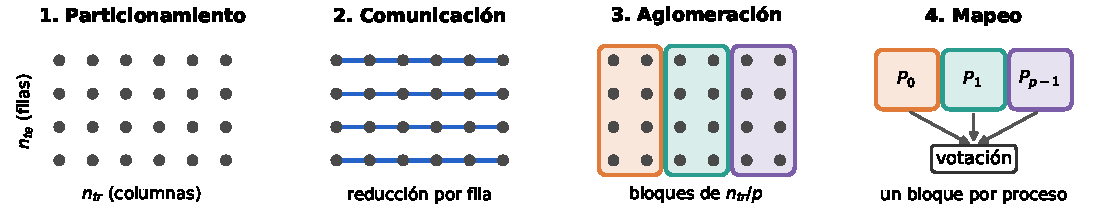
\includegraphics[width=0.92\textwidth]{figuras/F0_foster.pdf}
\caption{Método de Foster aplicado al KNN. Cada punto es una tarea: la distancia entre un punto de prueba (fila) y uno de entrenamiento (columna). Fuente: elaboración propia.}
\label{fig:foster}
\end{figure}

\subsection{PRAM: trabajo y span}
\label{sec:pram}

El Algoritmo~\ref{alg:pram} es el KNN en el modelo PRAM, sin ninguna referencia a $p$: se supone un procesador por tarea. Así el trabajo y el span se leen directamente del pseudocódigo. El modelo es CREW: todos los procesadores leen los mismos datos y cada uno escribe en su propia posición. Para que las dos reducciones en árbol (pasos 3 y 6) queden exactas suponemos, como en el ejemplo de la suma de $n$ números del curso [5], que $\ntr$ y $\nte$ son potencias de 2; si no lo son, se completan con posiciones vacías ($C[i, j] = \emptyset$ y $A[i] = 0$), que no cambian el resultado y a lo más duplican cada tamaño. En el paso 3, si la unión tiene menos de $k$ índices, se conservan todos.

\begin{algorithm}[!htb]
\caption{KNN en PRAM$(X_{tr}, y_{tr}, X_{te}, y_{te}, k)$ --- sin $p$}
\label{alg:pram}
\KwEntrada{datos de entrenamiento $X_{tr}$ ($\ntr \times d$) con etiquetas $y_{tr}$; datos de prueba $X_{te}$ ($\nte \times d$) con etiquetas $y_{te}$; $k$ vecinos}
\KwSalida{etiquetas predichas $\hat{y}[1,\dots,\nte]$ y precisión (\textit{accuracy})}
\ParaPar{$(i, j) \in \{1,\dots,\nte\} \times \{1,\dots,\ntr\}$}{
  $D[i, j] \leftarrow \sqrt{\sum_{l=1}^{d}\left(X_{te}[i,l]-X_{tr}[j,l]\right)^2}$ \tcp*[r]{paso 1}
  $C[i, j] \leftarrow \{\,j\,\}$ \tcp*[r]{paso 2}
}
\For{$h \leftarrow 1$ \KwTo $\log_2 \ntr$}{
  \ParaPar{$(i, j) \in \{1,\dots,\nte\} \times \{1,\dots,\ntr/2^h\}$}{
    $C[i, j] \leftarrow$ los $k$ índices de menor $D[i,\cdot]$ en $C[i, 2j-1] \cup C[i, 2j]$ \tcp*[r]{paso 3}
  }
}
\ParaPar{$i \leftarrow 1$ \KwTo $\nte$}{
  $\hat{y}[i] \leftarrow$ etiqueta más frecuente entre las $y_{tr}[j]$ con $j \in C[i, 1]$ \tcp*[r]{paso 4}
  $A[i] \leftarrow 1$ si $\hat{y}[i] = y_{te}[i]$, si no $0$ \tcp*[r]{paso 5}
}
\For{$h \leftarrow 1$ \KwTo $\log_2 \nte$}{
  \ParaPar{$i \leftarrow 1$ \KwTo $\nte/2^h$}{
    $A[i] \leftarrow A[2i-1] + A[2i]$ \tcp*[r]{paso 6}
  }
}
$accuracy \leftarrow A[1] \,/\, \nte$ \tcp*[r]{paso 7}
\Return{$\hat{y}, accuracy$}
\end{algorithm}

\textbf{Trabajo.} Contamos las operaciones paso por paso, como en el ejemplo de la suma de $n$ números del curso [5]. En los pasos 1 y 2 se ejecutan $\ntr\nte$ distancias de $3d$ operaciones y $\ntr\nte$ inicializaciones; en el paso 3, $\sum_{h=1}^{\log_2 \ntr} \nte\,\ntr/2^h$ mezclas de $O(k)$; en los pasos 4 y 5, $\nte$ votaciones entre $k$ y $\nte$ comparaciones; en el paso 6, $\sum_{h=1}^{\log_2 \nte} \nte/2^h$ sumas; y en el paso 7, una división. Como $\sum_{h\ge 1} \ntr/2^h < \ntr$ y $d$ y $k$ son constantes,
\[
W(n) = O(\ntr\,\nte\,d + k\,\ntr\,\nte + \nte\,k + \nte) = O(\ntr\,\nte) = O(n^2),
\]
que es el costo del mejor algoritmo secuencial (Sección~\ref{sec:secuencial}): el PRAM no ordena, solo mezcla listas de $k$.

\textbf{Span.} Los \textit{pardo} cuentan un paso y los \textit{for} secuenciales multiplican [5]: los pasos 1 y 2 cuestan un paso, el bucle del paso 3 cuesta $\log_2 \ntr$, los pasos 4 y 5 uno, el bucle del paso 6 cuesta $\log_2 \nte$ y el paso 7 uno. Dentro de cada paso, un solo procesador hace la suma de los $d$ términos de una distancia, la votación entre $k$ etiquetas o la mezcla de dos listas de $k$, en $O(d)$, $O(k)$ y $O(k)$ operaciones, o sea $O(1)$ porque $d = 64$ y $k = 3$ son constantes. Entonces
\[
T_\infty(n) = O(\log \ntr + \log \nte + 3) = O(\log n).
\]

\textbf{Brent.} Con $W$ y $T_\infty$, el tiempo con $p$ procesadores cumple [5]
\[
T_p(n,p) = O\!\left(\frac{W(n)}{p} + T_\infty(n)\right) = O\!\left(\frac{n^2}{p} + \log n\right),
\]
es decir, el algoritmo es casi perfectamente paralelo: el span es logarítmico y el trabajo se reparte. El costo es $C_p(n,p) = p\,T_p(n,p) = O(W(n) + p\,T_\infty(n)) = O(n^2 + p\log n)$, así que el algoritmo es de costo óptimo ($C_p = \Theta(W)$, el costo del mejor secuencial) mientras $p = O(n^2/\log n)$ [5]: con los tamaños y los $p \le 8$ que usamos, eso se cumple de sobra. Brent supone que no hay costo de comunicación [5]; la Sección~\ref{sec:dag} agrega ese costo.

\subsection{Algoritmo distribuido (el del DAG)}
\label{sec:dag}

El Algoritmo~\ref{alg:knn} es la versión con $p$ procesos que sigue el DAG del enunciado, y es la aglomeración descrita en la Sección~\ref{sec:foster}. Las líneas 1, 2 y 9 son \texttt{comm.bcast}, \texttt{comm.scatter} y \texttt{comm.gather}.

\begin{algorithm}[!htb]
\caption{KNN distribuido con Broadcast/Scatter/Gather$(X_{tr}, y_{tr}, X_{te}, y_{te}, k, p)$}
\label{alg:knn}
\KwEntrada{datos de entrenamiento $X_{tr}$ ($\ntr \times d$) con etiquetas $y_{tr}$; datos de prueba $X_{te}$ ($\nte \times d$) con etiquetas $y_{te}$; $k$ vecinos; $p$ procesos, $q$ el ID del proceso ($0 \le q \le p-1$)}
\KwSalida{etiquetas predichas $\hat{y}[1,\dots,\nte]$ y precisión (\textit{accuracy}) en el proceso 0}
Broadcast$(X_{te}, k, root = 0)$ \tcp*[r]{paso 1}
Scatter$((X_{tr}, y_{tr}), (X_q, y_q), root = 0)$ \tcp*[r]{paso 2}
\ParaPar{$q \leftarrow 0$ \KwTo $p-1$}{
  \For{$i = 1$ \KwTo $\nte$}{
    \For{$j = 1$ \KwTo $\ntr/p$}{
      $D[j] \leftarrow \sqrt{\sum_{l=1}^{d}\left(X_{te}[i,l]-X_q[j,l]\right)^2}$ \tcp*[r]{paso 3}
    }
    $I \leftarrow$ índices de los $k$ menores valores de $D$ (ordenar $D$) \tcp*[r]{paso 4}
    $C_q[i] \leftarrow \{(D[j], y_q[j]) : j \in I\}$\;
  }
}
Gather$(C_q, C, root = 0)$ \tcp*[r]{paso 5}
\If{$q = 0$}{
  \For(\tcp*[f]{paso 6}){$i = 1$ \KwTo $\nte$}{
    $V \leftarrow$ los $k$ pares de menor distancia en $C[i]$\;
    $\hat{y}[i] \leftarrow$ etiqueta más frecuente en $V$\;
  }
  $accuracy \leftarrow$ (cantidad de $i$ con $\hat{y}[i] = y_{te}[i]$) $/\ \nte$ \tcp*[r]{paso 7}
  \Return{$\hat{y}, accuracy$}
}
\end{algorithm}

Usamos el modelo de comunicación del curso [5], con $a \equiv \alpha$ (latencia) y $b \equiv \beta$ (tiempo por dato) como en el DAG. El DAG del enunciado usa una topología lineal, en la que el scatter y el gather de $m$ datos cuestan $O(a\,p + b\,m)$: pagan $p$ veces la latencia, y es una aproximación no optimizada. MPI organiza las colectivas en árbol. Así, el broadcast cuesta $O(\log p\,(a + m\,b))$, y el scatter y el gather $O(a\log p + b\,m)$: la latencia se paga en $\log p$ niveles, pero el maestro igual envía o recibe los $m$ datos [5]. Así nos lo aclaró el profesor [10], y con esos costos, escritos con un solo $n$, queda la Tabla~\ref{tab:pasos}. En el DAG el gather cuesta $O(p(a + k\,b))$, que es el costo para un punto de prueba; nosotros hacemos un solo Gather con los candidatos de los $\nte$ puntos (para no repetir la latencia $\nte$ veces), así que el maestro recibe $m = p\,\nte\,k$ pares. $T_{comp_2}$ no aparece en el DAG, pero es el trabajo de su último nodo (votación), que hace el maestro.

\begin{table}[!htb]
\centering
\small
\renewcommand{\arraystretch}{1.2}
\begin{tabular}{c c >{\raggedright\arraybackslash}p{5.2cm} l}
\toprule
\textbf{Paso} & \textbf{Líneas} & \textbf{Qué se ejecuta} & \textbf{Costo} \\
\midrule
1 & 1 & Broadcast de los $0{,}2n$ datos de prueba & $T_{comm_1} = O(\log(p)(a + n\, b))$ \\
2 & 2 & Scatter de $0{,}8n/p$ datos a cada proceso & $T_{comm_2} = O(a\log p + n\, b)$ \\
3 y 4 & 3--8 & $0{,}16\,n^2/p$ distancias y ordenamiento & $T_{comp_1} = O\big(\frac{n^2}{p}(d + \log \frac{n}{p})\big) \approx O\big(\frac{n^2}{p}\big)$ \\
5 & 9 & Gather de $k$ candidatos por punto de prueba & $T_{comm_3} = O(a\log p + n\, k\, p\, b)$ \\
6 y 7 & 10--15 & Selección de $k$ entre $p \cdot k$, votación y precisión & $T_{comp_2} = O(n\, p\, k)$ \\
\bottomrule
\end{tabular}
\caption{Costo de cada paso del Algoritmo~\ref{alg:knn}, con $\ntr = 0{,}8n$ y $\nte = 0{,}2n$. La aproximación de $T_{comp_1}$ vale mientras $\log_2(n/p) < d$.}
\label{tab:pasos}
\end{table}

Sumando los pasos, y con $S = T_s/T_p$ y $E = S/p$ [5]:
\begin{align*}
T_p(n,p) &= O\Big(\frac{n^2}{p} + n\, k\, p + a\log p + b\,\big(n + n \log p + n\, k\, p\big)\Big)\\
E(n,p) &= O\left(\frac{1}{1 + \dfrac{k\,p^2}{n} + \dfrac{p \log p}{n} + \dfrac{p}{n} + \dfrac{p\log p}{n^2}}\right)
 = O\left(\frac{1}{1 + \dfrac{k\,p^2}{n}}\right)
\end{align*}
En el último paso quitamos los términos menores: $p/n \le k\,p^2/n$ y $p\log p/n \le k\,p^2/n$ (porque $1 \le k\,p$ y $\log_2 p \le k\,p$ con $k \ge 1$), y $p\log p/n^2 \le k\,p^2/n$. Queda un solo término de \textit{overhead}, $k\,p^2/n$, que viene del gather de los candidatos y de la mezcla en el maestro: la eficiencia se mantiene alta mientras $n \gg k\,p^2$.

\subsection{Código en mpi4py}

El Listado~\ref{lst:codigo} muestra la parte central de la versión final. Las colectivas van en minúscula (objetos de Python), con \texttt{root=0}. Como $\ntr$ no es múltiplo de $p$, el maestro reparte con \texttt{np.array\_split}, que deja bloques que difieren en a lo más una fila. Cada candidato lleva su índice global para desempatar distancias iguales en el paso 6.

\begin{lstlisting}[caption={Parte central de \texttt{knn\_mpi\_beta3.py} simplificada: sin las barreras ni las marcas de tiempo intermedias de la medición (los pasos corresponden al Algoritmo~\ref{alg:knn}).}, label={lst:codigo}]
t0 = MPI.Wtime()
X_te, k_l = comm.bcast((X_test, k), root=0)          # 1. Broadcast de la data de prueba
if rank == 0:                                        # 2. Scatter de la data de entrenamiento
    idx = np.arange(len(X_train))
    bloques = list(zip(np.array_split(X_train, size),
                       np.array_split(y_train, size),
                       np.array_split(idx, size)))
else:
    bloques = None
X_q, y_q, idx_q = comm.scatter(bloques, root=0)
C_q = k_vecinos_locales(X_te, X_q, y_q, idx_q, k_l)  # 3-4. k vecinos locales
C = comm.gather(C_q, root=0)                         # 5. Gather de los candidatos
# beta 3b: C = comm.reduce(C_q, op=mezcla, root=0)   # 5-6. reduccion en arbol
if rank == 0:
    y_pred = mezclar_y_votar(C, k_l)                 # 6. k globales y votacion
    # beta 3b: y_pred = votar(C[1])                  # 6. solo la votacion
    acc = np.mean(y_pred == y_test)                  # 7. Precision
tf = MPI.Wtime()
\end{lstlisting}

\subsection{Versiones beta y validación}
\label{sec:validacion}

Las tres versiones tienen la misma estructura (el DAG y el Algoritmo~\ref{alg:knn}); lo que cambia es cómo se calcula el cómputo local:
\begin{itemize}[nosep]
  \item \textbf{Beta 1:} traducción directa del Algoritmo~\ref{alg:knn}. Las distancias se calculan como en el código base, con un bucle de Python y \texttt{euclidean\_distance} por cada par.
  \item \textbf{Beta 2:} para cada punto de prueba se calculan con NumPy todas las distancias al bloque local en una sola operación; la mezcla y la votación del maestro también se vectorizan. Con ella empezamos a medir por fases y a guardar las repeticiones en un archivo CSV; para la entrega final, las tres betas se miden con el mismo protocolo.
  \item \textbf{Beta 3 (final):} la matriz de distancias de un bloque de hasta 512 puntos de prueba se calcula con $\|x-y\|^2 = \|x\|^2 + \|y\|^2 - 2\,x\cdot y$, que es la misma distancia pero usa un producto de matrices. Se agrega el tamaño variable del problema y la versión secuencial del mismo cálculo (para $T_s$).
  \item \textbf{Beta 3b (mejora):} igual a la beta 3, pero el gather de los candidatos y la mezcla del maestro se reemplazan por \texttt{comm.reduce} con una operación que deja los $k$ menores de dos listas; así la mezcla se hace en árbol, en $\log_2 p$ niveles (Sección~\ref{sec:mejoras}).
\end{itemize}

\textbf{Validación.} Como el código lo escribió una herramienta de IA [9], lo validamos comparando las predicciones (\texttt{validar.py}, 49 casos). Con los datos originales, las betas 1, 2, 3 y 3b dan exactamente las mismas 360 predicciones que el código base para $p = 1$ a $8$, con precisión 0,9833 (Tabla~\ref{tab:betas}). Con $n/4$ y $4n$ ($p = 4$ y $8$), las betas 3 y 3b dan las mismas predicciones que el código base y que la versión secuencial de la beta 3, y en la serie débil también la beta 3; con $16n$ ($p = 8$), las dos dan las mismas que la secuencial. También probamos bloques con menos de $k$ puntos ($\ntr = 7$ con $p = 8$), que se completan con candidatos de distancia infinita. En 7 de los 360 puntos de prueba hay un empate de distancia en el tercer vecino (\texttt{pruebas\_extra.py}); el desempate por índice global puede elegir otro vecino que \texttt{np.argsort}, pero las predicciones siguen siendo las mismas, como muestra la validación. El código, los scripts y los datos medidos van en el .zip adjunto (ver \texttt{README.md}).

\begin{table}[!htb]
\centering
\small
\begin{tabular}{lcccc}
\toprule
\textbf{Versión} & \textbf{Accuracy} & $\mathbf{T_{ej}(p{=}1)}$ \textbf{(ms)} & $\mathbf{T_{ej}(p{=}8)}$ \textbf{(ms)} & $\mathbf{T(1)/T(8)}$ \\
\midrule
beta 1 & 0,9833 & 1034,1 & 164,9 & 6,27 \\
beta 2 & 0,9833 & 53,9 & 10,3 & 5,24 \\
beta 3 & 0,9833 & 27,0 & 3,7 & 7,21 \\
beta 3b & 0,9833 & 26,6 & 3,8 & 7,05 \\
\bottomrule
\end{tabular}
\caption{Versiones beta con los datos originales ($n = 1797$), mediana de 4 repeticiones. $T_{ej}$ es el tiempo de la región paralelizable, definido en la Sección~\ref{sec:experimental}. En todas, las predicciones son iguales a las del código base para $p = 1$ a $8$. El código base tarda 1024 ms.}
\label{tab:betas}
\end{table}

\subsection{Diseño experimental}
\label{sec:experimental}

\textbf{Entorno.} El clúster Khipu no estuvo disponible por un problema de \textit{firewall} de la universidad; el profesor indicó que en ese caso estaba justificado medir en una computadora personal [10]. Medimos en una Apple M1 Pro con 10 núcleos (8 de rendimiento y 2 de eficiencia) y 16 GB de RAM, con macOS 27.2.1, Python 3.11.6, NumPy 2.4.6, scikit-learn 1.9.1, mpi4py 4.1.2 y Open MPI 5.0.11, todo en una sola sesión de 33 min. Usamos $p \le 8$ para que haya a lo más un proceso MPI por núcleo de rendimiento [7]; macOS no permite fijar cada proceso a un núcleo, así que el sistema operativo decide dónde corre cada uno. Cada proceso usa un solo hilo (\texttt{OMP\_NUM\_THREADS=1}, \texttt{VECLIB\_MAXIMUM\_THREADS=1}). Cerramos OneDrive, Docker y las aplicaciones que no hacían falta. La sesión fue a batería (sin modo de bajo consumo) y con Claude Code abierto, que lanzó el barrido; su uso de CPU queda dentro de la carga externa. Antes de cada corrida registramos la carga externa, es decir, los núcleos que usaban otros programas (mediana 0,9; máximo 3,5), y en cada corrida el menor cociente entre tiempo de CPU y tiempo real de los procesos (mediana 0,996). Ese cociente fue menor que 0,9 en 18 de 490 corridas, 15 de ellas con $p = 8$: ahí otro programa le quitó CPU a algún proceso.

\textbf{Tamaños del problema.} Además de los datos originales ($n_0$), usamos un subconjunto ($n/4$: las primeras filas de cada parte) y dos tamaños mayores ($4n$ y $16n$); los nombres $n/4$, $4n$ y $16n$ son siempre relativos a $n_0$. Para crecer hicimos réplicas de las imágenes con ruido gaussiano ($\sigma = 1$ píxel, semilla fija) después del \textit{split} del código base, sin mezclar entrenamiento con prueba; así se mantienen $d = 64$, la proporción 80/20 y una precisión con sentido (Tabla~\ref{tab:tamanos} y Figura~\ref{fig:precision}). El profesor también usa datos sintéticos para escalar el KNN (\texttt{knn.cpp}, 20\,000/5000 puntos [8]). Como la proporción 80/20 se mantiene, cada tamaño queda descrito por un solo $n$.

\textbf{Series de escalabilidad.} Además de las series con $n$ fijo (escalabilidad fuerte), medimos dos series donde $n$ crece con $p$: la \textbf{débil}, con $n \propto \sqrt{p}$, que deja constante el trabajo por proceso ($W/p = 0{,}16\,n^2/p$), y la de \textbf{isoeficiencia}, con $n \propto k\,p^2$, que es la condición de la Sección~\ref{sec:esc}. Las réplicas admiten factores no enteros, así que $n$ puede crecer como $\sqrt{p}$. Medimos además una serie de \textbf{control} con $\nte$ fijo y $\ntr \propto p$ (dos $n$ separados): ahí el trabajo por proceso también es constante, pero el largo de las listas que ordena cada proceso no cambia, así que sirve para aislar el efecto del hardware compartido (Sección~\ref{sec:dif}).

\begin{table}[!htb]
\centering
\small
\begin{tabular}{lrrrccr}
\toprule
\textbf{Tamaño} & $\mathbf{\ntr}$ & $\mathbf{\nte}$ & \textbf{Pares} & \textbf{FLOP} & \textbf{Accuracy} & $\mathbf{T_s}$ \textbf{(ms)} \\
\midrule
$n/4$ & 359 & 90 & 32\,310 & $6{,}20\cdot 10^{6}$ & 0,9778 & 1,21 \\
$n_0$ & 1\,437 & 360 & 517\,320 & $9{,}93\cdot 10^{7}$ & 0,9833 & 26,81 \\
$4n$ & 5\,748 & 1\,440 & 8\,277\,120 & $1{,}59\cdot 10^{9}$ & 0,9812 & 517,97 \\
$16n$ & 22\,992 & 5\,760 & 132\,433\,920 & $2{,}54\cdot 10^{10}$ & 0,9807 & 9754,85 \\
\bottomrule
\end{tabular}
\caption{Tamaños del problema. FLOP $= 3d\cdot\ntr\cdot\nte$; $T_s$ es la versión secuencial de la beta 3 (mediana).}
\label{tab:tamanos}
\end{table}

\begin{figure}[!htb]
\centering
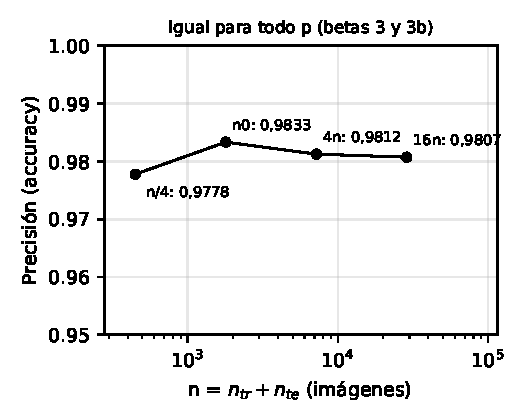
\includegraphics[width=0.45\textwidth]{figuras/F10_precision.pdf}
\caption{Precisión de cada tamaño del problema; es la misma para todo $p$ y en las betas 3 y 3b. Fuente: elaboración propia.}
\label{fig:precision}
\end{figure}

\textbf{Medición.} Medimos con \texttt{MPI.Wtime()} en el maestro, desde antes del broadcast hasta después de calcular la precisión (la carga y la división de los datos quedan fuera, como en el código base). Cada \texttt{mpirun} mide una sola repetición de una configuración, y el script recorre toda la malla repetición por repetición (en las impares, en orden inverso). Así las repeticiones de una misma configuración quedan separadas en el tiempo, y una racha de carga no afecta siempre a la misma. Hicimos 4 repeticiones (2 en el tamaño mayor de isoeficiencia, cuya versión secuencial tarda 3 min) y reportamos la mediana; las barras de las figuras van de la repetición más rápida a la más lenta. Antes de medir, cada \texttt{mpirun} corre rondas de calentamiento que se descartan hasta juntar unos 0,25 s (entre 1 y 30 rondas; ninguna en los tamaños de más de $2\cdot 10^8$ pares). Las configuraciones que se repiten en varias series (por ejemplo, $n_0$ con $p = 1$) se miden una sola vez, así que todas las series comparten la misma línea base. Hicimos dos modos: en el modo A no hay barreras dentro de la región medida y de ahí sale $T_{ej}$ (con el que calculamos $S$, $E$ y FLOP/s); en el modo B ponemos \texttt{comm.Barrier()} antes de cada marca solo para separar las fases, porque sin barreras el gather incluiría la espera del proceso más lento. Los dos modos se miden en el mismo \texttt{mpirun}, en orden alternado. Definimos $T_{comm} = T_{bcast} + T_{scatter} + T_{gather}$ y $T_{comp} = T_{comp_1} + T_{comp_2}$, con $T_{comp_1}$ el del proceso más lento. Como $T_s$ usamos la versión secuencial del mismo cálculo de la beta 3, medida de la misma forma. No es el mejor algoritmo secuencial [8]: con selección de los $k$ menores (\texttt{np.argpartition}) sería más rápido y $S$ sería menor (Secciones~\ref{sec:speedup} y \ref{sec:mejoras}); la usamos para que $S$ compare el mismo cálculo repartido entre $p$ procesos.

\subsection{FLOP de la región paralelizable}

La región paralelizable es el cálculo de distancias entre los puntos de prueba y los de entrenamiento. Según la fórmula de la distancia euclidiana, cada par necesita $d$ restas, $d$ productos, $d-1$ sumas y una raíz; contando todas las operaciones igual [8]:
\[
\text{FLOP por par} = 3d = 192, \qquad \text{FLOP}_{total} = 3d\,\ntr\,\nte = 99\,325\,440 \ \text{ con los datos originales.}
\]
Usamos este mismo conteo en las tres versiones, aunque la beta 3 calcule la distancia con un producto de matrices, para que las tasas sean comparables. La velocidad es FLOP/s $= \text{FLOP}_{total}/T_{ej}$ [8].

%====================================================================
\section{Resultados y análisis}

\subsection{Tiempos de ejecución, cómputo y comunicación}
\label{sec:tiempos}

La Figura~\ref{fig:tiempos} muestra $T_{ej}$, $T_{comp}$ y $T_{comm}$ para los cuatro tamaños, y la Tabla~\ref{tab:res} los valores para $n_0$ y $16n$. El cómputo baja casi como $1/p$, y la comunicación crece poco con $p$: en $16n$ sube de 3,7 a 10,0 ms, y en $n_0$ se mantiene entre 0,42 y 0,53 ms hasta $p = 6$ y llega a 0,65 ms con $p = 8$, porque la domina el scatter, cuyo término de datos no depende de $p$. Para $4n$ y $16n$ la comunicación es entre 27 y 2700 veces menor que el cómputo (granularidad $G = T_{comp}/T_{comm}$ [5]), así que el problema es \textit{compute bound} en todo el rango. Para $n/4$, en cambio, con $p = 8$ la comunicación ya es casi igual al cómputo ($G \approx 1{,}2$) y el tiempo total vuelve a subir. La precisión de cada tamaño es la misma para todo $p$ (Figura~\ref{fig:precision}).

\begin{figure}[!htb]
\centering
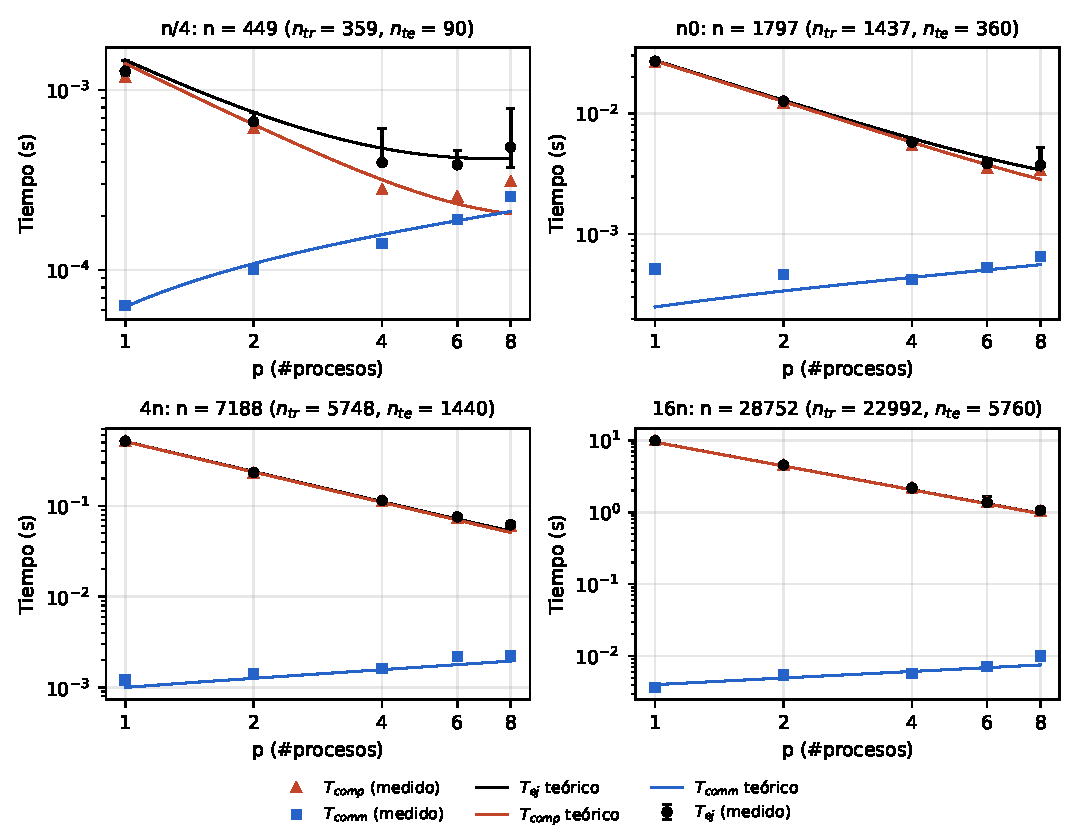
\includegraphics[width=0.92\textwidth]{figuras/F1_tiempos.pdf}
\caption{Tiempos de ejecución, cómputo y comunicación medidos (marcadores: mediana; barras: mínimo y máximo) y modelo teórico normalizado (líneas), para cada tamaño. Fuente: elaboración propia.}
\label{fig:tiempos}
\end{figure}

\begin{table}[!htb]
\centering
\small
\setlength{\tabcolsep}{4pt}
\begin{tabular}{rrrrrrrrrr}
\toprule
$p$ & $T_{ej}$ (ms) & $T_{comp}$ (ms) & $T_{comm}$ (ms) & $G$ & $S$ & $E$ & $\Delta T/\Delta p$ & GFLOP/s & desbal. \\
\midrule
\multicolumn{10}{l}{\textit{$n_0$: $\ntr = 1437$, $\nte = 360$}} \\
1 & 26,96 $\pm$ 0,99 & 26,26 & 0,52 & 50,9 & 0,99 & 0,99 & -- & 3,68 & 1,00 \\
2 & 12,61 $\pm$ 0,05 & 12,15 & 0,46 & 26,4 & 2,13 & 1,06 & -14,35 & 7,87 & 1,01 \\
4 & 5,76 $\pm$ 0,08 & 5,41 & 0,42 & 12,8 & 4,65 & 1,16 & -3,42 & 17,23 & 1,02 \\
6 & 3,83 $\pm$ 0,24 & 3,51 & 0,53 & 6,6 & 7,00 & 1,17 & -0,97 & 25,92 & 1,05 \\
8 & 3,74 $\pm$ 1,03 & 3,36 & 0,65 & 5,1 & 7,17 & 0,90 & -0,05 & 26,56 & 1,22 \\
\midrule
\multicolumn{10}{l}{\textit{$16n$: $\ntr = 22\,992$, $\nte = 5760$}} \\
1 & 9832,40 $\pm$ 138,11 & 9859,61 & 3,66 & 2695,7 & 0,99 & 0,99 & -- & 2,59 & 1,00 \\
2 & 4522,13 $\pm$ 116,41 & 4518,00 & 5,41 & 834,7 & 2,16 & 1,08 & -5310,27 & 5,62 & 1,01 \\
4 & 2165,59 $\pm$ 28,59 & 2153,61 & 5,74 & 375,4 & 4,50 & 1,13 & -1178,27 & 11,74 & 1,01 \\
6 & 1355,78 $\pm$ 167,83 & 1357,21 & 7,21 & 188,3 & 7,20 & 1,20 & -404,90 & 18,75 & 1,01 \\
8 & 1055,70 $\pm$ 34,53 & 1024,92 & 9,99 & 102,6 & 9,24 & 1,16 & -150,04 & 24,09 & 1,02 \\
\bottomrule
\end{tabular}
\caption{Resultados por $p$: mediana de 4 repeticiones; $\pm$ es la mitad del rango entre la más rápida y la más lenta. $\Delta T/\Delta p$ en ms por proceso; desbalance = máximo entre promedio de $T_{comp_1,q}$.}
\label{tab:res}
\end{table}

La Figura~\ref{fig:colectivas} separa las tres colectivas. El scatter es la más cara porque el maestro envía todo el entrenamiento ($\ntr\, b$, casi constante en $p$); el broadcast crece como $\log p$, y el gather crece con $p$ porque el maestro recibe $p\,\nte\,k$ candidatos. Las latencias se ajustan con $\log p$, como en MPI (Sección~\ref{sec:dag}). Todos estos tiempos son del orden de $10^{-4}$ a $10^{-2}$ s, así que tienen más ruido relativo que el cómputo.

\begin{figure}[!htb]
\centering
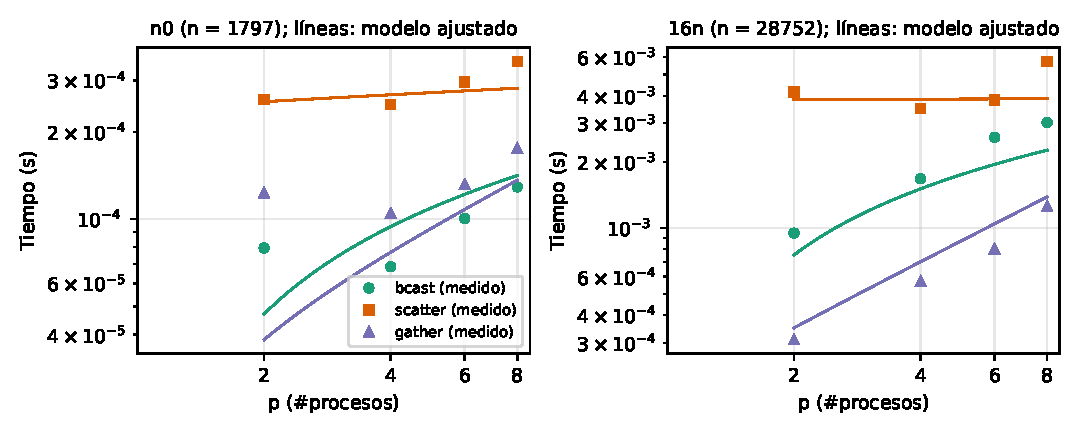
\includegraphics[width=0.88\textwidth]{figuras/F2_colectivas.pdf}
\caption{Tiempo de cada colectiva (modo B) y su modelo ajustado. Fuente: elaboración propia.}
\label{fig:colectivas}
\end{figure}

\subsection{Comparación de las versiones beta}

Con los datos originales, pasar del bucle de Python (beta 1) a NumPy (beta 2) reduce el tiempo 19 veces, y el producto de matrices (beta 3) lo reduce otras 2 veces (Figura~\ref{fig:betas}). La beta 3 con un proceso tarda 27,0 ms frente a 1024 ms del código base. El orden del algoritmo es el mismo en las tres; lo que cambia es la constante de cada operación. En \textit{speedup} relativo, la beta 1 (6,3 con $p = 8$) supera a la beta 2 (5,2) porque el cómputo local de la beta 2 se reparte peor con $p = 8$: su proceso más lento tarda 1,2 veces el promedio (1,05 en la beta 1), y con cómputos de pocos ms cualquier interrupción pesa más. La comunicación pesa lo mismo en las dos (5,6\,\% del tiempo en el modo B). La beta 3 llega a 7,2 porque además su costo por par baja con $\log_2(\ntr/p)$ (Sección~\ref{sec:speedup}).

\begin{figure}[!htb]
\centering
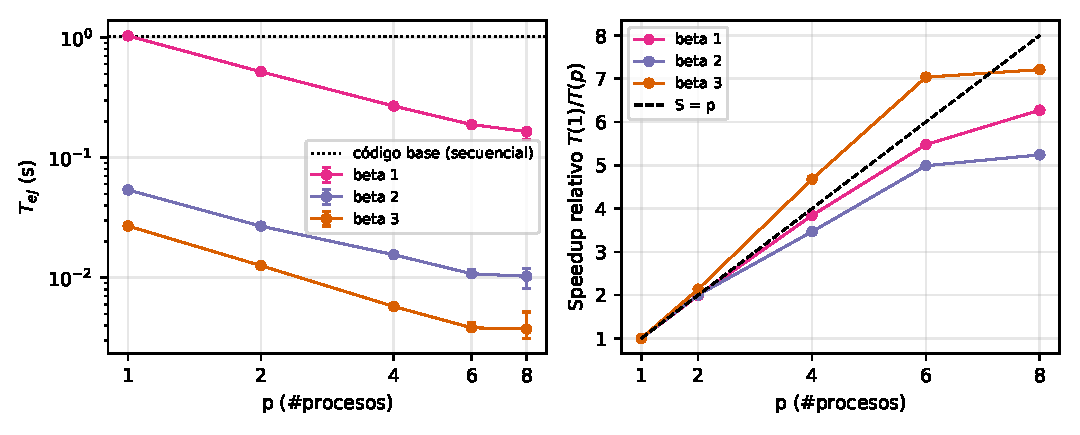
\includegraphics[width=0.88\textwidth]{figuras/F8_betas.pdf}
\caption{Versiones beta con $n = 1797$: tiempo de ejecución y \textit{speedup} relativo $T(1)/T(p)$. Fuente: elaboración propia.}
\label{fig:betas}
\end{figure}

\subsection{Normalización de la expresión teórica}
\label{sec:norma}

Para comparar la expresión $O(\cdot)$ con los tiempos medidos, multiplicamos cada término por una constante física, de la misma forma que $T_{CPU} = n_{instr}\cdot CPI\cdot t_{cycle}$ y $T(m) = \alpha + m\beta$ [8]:
\begin{align*}
T_p^{teo}(n,p) = {}& \underbrace{\nte\frac{\ntr}{p}\Big(c_d + c_s\log_2\frac{\ntr}{p}\Big)}_{T_{comp_1}} + \underbrace{c_2\,\nte\,k\,p}_{T_{comp_2}} + \underbrace{\log_2 p\,(a_1 + \nte b_1)}_{\text{bcast}}\\
&+ \underbrace{a_2\log_2 p + \ntr b_2}_{\text{scatter}} + \underbrace{a_3\log_2 p + p\,\nte k\, b_3}_{\text{gather}}
\end{align*}
Cada constante la obtuvimos de su propia fase medida en el modo B (Tabla~\ref{tab:const}), con mínimos cuadrados ponderados por el error relativo: para $T_{comp_1}$ usamos todos los $(n,p)$ y para las colectivas solo $p \ge 2$ (con $p = 1$ no hay mensajes entre procesos); $c_2$ es la mediana de $T_{comp_2}/(\nte k p)$. En el ajuste del broadcast, $a_1$ salió negativo; como no tiene sentido físico, lo fijamos en 0 y volvimos a ajustar $b_1$. No usamos el tiempo total para ajustar, así que la comparación con $T_{ej}$ sirve para validar el modelo, aunque no es del todo independiente: los modos A y B se miden en la misma ejecución.

\begin{table}[!htb]
\centering
\small
\begin{tabular}{llll}
\toprule
\textbf{Constante} & \textbf{Término} & \textbf{Valor} & \textbf{Se obtiene de} \\
\midrule
$c_s$ & ordenamiento (paso 4) & 4,64 ns por par y nivel & $T_{comp_1}$ medido \\
$c_d$ & distancias (paso 3) & 3,79 ns por par & $T_{comp_1}$ medido \\
$c_2$ & mezcla y votación (paso 6) & 41 ns por candidato & $T_{comp_2}$ medido \\
$a_1$, $b_1$ & broadcast & 0 (ajuste libre $<0$); 0,131 $\mu$s/dato (512 B) & $T_{bcast}$ medido \\
$a_2$, $b_2$ & scatter & 14,3 $\mu$s por nivel; 0,167 $\mu$s/dato (512 B) & $T_{scatter}$ medido \\
$a_3$, $b_3$ & gather & 17,6 $\mu$s por nivel; 9,6 ns/candidato (24 B) & $T_{gather}$ medido \\
\bottomrule
\end{tabular}
\caption{Constantes de la normalización (beta 3).}
\label{tab:const}
\end{table}

\begin{table}[!htb]
\centering
\small
\begin{tabular}{lrrrr}
\toprule
\textbf{Variante} & $\boldsymbol{\alpha}$ ($\mu$s) & $\boldsymbol{\beta}$ (ns/dato) & \textbf{GB/s} & \textbf{Error máx.} \\
\midrule
búfer (\texttt{Send}/\texttt{Recv}) & 0,52 & 0,425 & 18,8 & 68\,\% \\
objetos (\texttt{send}/\texttt{recv}, \textit{pickle}) & 5,28 & 1,975 & 4,1 & 119\,\% \\
\bottomrule
\end{tabular}
\caption{Ping-pong entre dos procesos, $T(m) = \alpha + m\,\beta$ con $m$ datos \textit{float64}: $\alpha$ es la mediana con $m \le 100$ y $\beta$ la pendiente con $m \ge 10^4$. El error máximo de la recta es grande porque el costo por dato cambia con el tamaño del mensaje (caché).}
\label{tab:pingpong}
\end{table}

Las dos constantes del cómputo local quedan cerca de lo que mide la prueba aparte (\texttt{pruebas\_\allowbreak extra.py}): $c_d = 3{,}8$ frente a 5,2 ns por par para las distancias, y $c_s = 4{,}6$ frente a 4,4 ns por par y nivel para el ordenamiento.

El modelo normalizado reproduce $T_{ej}$ con $R^2 = 0{,}998$ y un error relativo medio de 8\,\% (5--6\,\% para $n_0$, $4n$ y $16n$; 14\,\% para $n/4$, donde los tiempos son de 1,3 ms o menos y el ruido pesa más). Dos resultados del ajuste son importantes:
\begin{itemize}[nosep]
  \item \textbf{El ordenamiento domina el cómputo local.} En el PRAM supusimos que las distancias pesan más que el ordenamiento porque $d = 64 > \log_2\ntr$. Eso vale para la beta 1, pero en la beta 3 las distancias salen de un producto de matrices: en una prueba aparte con un proceso (\texttt{pruebas\_extra.py}), el paso 3 cuesta 5,2 ns por par y el paso 4 (ordenar) 46,4 ns por par, es decir 4,4 ns por nivel de $\log_2\ntr$. El ordenamiento es cerca del 90\,\% del cómputo local, y por eso el costo por par crece con $\log_2(\ntr/p)$ (Figura~\ref{fig:costopar}). El orden del paso 3--4 es el de la Tabla~\ref{tab:pasos}, $O(\nte\,(\ntr/p)(d + \log(\ntr/p)))$; lo que cambió es cuál de los dos términos pesa.
  \item \textbf{Latencias y costo por dato.} Medimos el tiempo de un mensaje entre dos procesos con un ping-pong (\texttt{ping\_pong.py}, Tabla~\ref{tab:pingpong}). Con objetos de Python (\textit{pickle}, como las colectivas en minúscula), $\alpha = 5{,}3\ \mu$s y $\beta = 2{,}0$ ns por \textit{float64}; con búferes de NumPy, $\alpha = 0{,}5\ \mu$s y $\beta = 0{,}43$ ns. Los costos por dato del ajuste coinciden con la variante con objetos: $b_1$, $b_2$ y $b_3$ equivalen a 2,0, 2,6 y 3,2 ns por valor. Las latencias por nivel del scatter y del gather (14 y 18 $\mu$s) son mayores que $\alpha$, porque cada colectiva arma y serializa los mensajes de todos los procesos. Las latencias quedan por encima del rango $10^{-7}$--$10^{-9}$ s que da el curso para $\alpha$ y $\beta$ [5], y el costo por byte ($\approx 0{,}25$--$0{,}40$ ns/B) por debajo, porque todos los procesos están en la misma computadora y los datos se copian por memoria.
\end{itemize}

\begin{figure}[!htb]
\centering
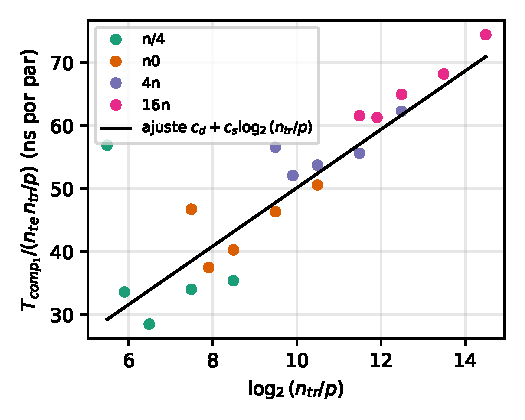
\includegraphics[width=0.45\textwidth]{figuras/F9_costo_por_par.pdf}
\caption{Costo del cómputo local por par prueba--entrenamiento en función de $\log_2(\ntr/p)$, para todos los $(n,p)$, y el ajuste. Fuente: elaboración propia.}
\label{fig:costopar}
\end{figure}

\subsection{Cantidad óptima de procesos}

Agrupando el modelo como $T(p) = A/p + B\,p + C\log_2 p + D$, con $A = \ntr\,\nte\,(c_d + c_s\log_2(\ntr/p))$, $B = c_2\nte k + \nte k\, b_3$ y $C = a_1 + a_2 + a_3 + \nte b_1$, y tomando $\log_2(\ntr/p)$ aproximadamente constante cerca del óptimo, el número óptimo de procesos se obtiene de [8]:
\[
T'(p) = -\frac{A}{p^2} + B + \frac{C}{p\ln 2} = 0 \;\Rightarrow\; p_{opt} = \frac{-C/\ln 2 + \sqrt{(C/\ln 2)^2 + 4AB}}{2B} \approx \sqrt{\frac{A}{B}}
\]
La segunda derivada en $p_{opt}$ es positiva ($p^2 T'' = 2Bp + C/\ln 2 > 0$), así que es un mínimo. Como $A \propto n^2$ y $B \propto n\,k$, $p_{opt}$ crece aproximadamente como $\sqrt{n/k}$ (en la Tabla~\ref{tab:popt}, algo más rápido, por el factor $\log$). Como la fórmula es aproximada, la Tabla~\ref{tab:popt} usa el mínimo numérico de $T_p^{teo}$. La tabla compara tres estimaciones: la de la expresión $T_p$ de la Sección~\ref{sec:dag} sin constantes ($a = b = 1$ y $t_c = 1$, con $t_c$ el tiempo de una distancia), la del modelo normalizado y la medida.

\begin{table}[!htb]
\centering
\small
\begin{tabular}{lrrccc}
\toprule
\textbf{Tamaño} & $\mathbf{\ntr}$ & $\mathbf{\nte}$ & $\mathbf{p_{opt}}$ \textbf{($a{=}b{=}t_c{=}1$)} & $\mathbf{p_{opt}}$ \textbf{(normalizado)} & \textbf{Mínimo medido ($p \le 8$)} \\
\midrule
$n/4$ & 359 & 90 & 7,6 & 7,3 & 6 \\
$n_0$ & 1\,437 & 360 & 15,4 & 18,4 & 8 \\
$4n$ & 5\,748 & 1\,440 & 30,8 & 40,1 & 8 \\
$16n$ & 22\,992 & 5\,760 & 61,8 & 84,9 & 8 \\
\bottomrule
\end{tabular}
\caption{Cantidad óptima de procesos.}
\label{tab:popt}
\end{table}

\begin{figure}[!htb]
\centering
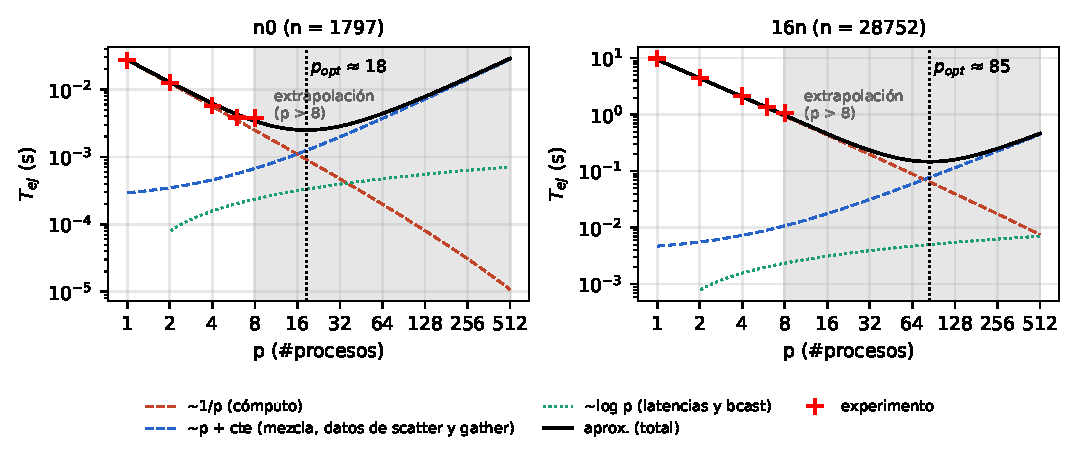
\includegraphics[width=0.92\textwidth]{figuras/F3_popt.pdf}
\caption{Modelo normalizado y sus términos (líneas) frente a las mediciones (cruces rojas) para $n_0$ y $16n$. La zona gris ($p > 8$) es extrapolación. Fuente: elaboración propia.}
\label{fig:popt}
\end{figure}

\textbf{Respuesta.} Para el problema del enunciado ($n = 1797$) estimamos $p_{opt} \approx 18$ procesos: hasta ahí el cómputo, que baja como $1/p$, pesa más que la mezcla del maestro y los datos del gather, que crecen como $p$ (Figura~\ref{fig:popt}). En nuestra computadora, con 8 núcleos de rendimiento, el mejor valor medido es $p = 8$, aunque pasar de 6 a 8 procesos solo ahorra 0,1 ms ($\Delta T/\Delta p = -0{,}05$ ms por proceso), así que en la práctica $p = 6$--$8$ es el punto razonable. Para $n/4$ el mínimo sí cae dentro del rango: el modelo da $p_{opt} \approx 7$ y el mínimo medido está en $p = 6$ (con $p = 4$ casi igual). Para $4n$ y $16n$ el modelo da $p_{opt} \approx 40$ y $85$, fuera de los 8 núcleos, por lo que en esos casos conviene usar todos los núcleos disponibles.

\subsection{Speedup y FLOP/s}
\label{sec:speedup}

La Figura~\ref{fig:speedup} muestra el \textit{speedup}, calculado con los tiempos $T_{ej}$ de la Sección~\ref{sec:tiempos}. Para $n/4$ el \textit{speedup} llega a 3,1 con $p = 6$ y luego baja, por el \textit{overhead}. Para $n_0$ llega a 7,2 con $p = 8$ y supera la recta $S = p$ con $p = 2$ a 6; para $4n$ y $16n$ la supera con todo $p \ge 2$ ($S = 9{,}2$ con $p = 8$ en $16n$). Un \textit{speedup} superlineal es raro [8]; aquí lo explica el término de ordenamiento: cada proceso ordena listas de $\ntr/p$ elementos, así que su costo por par baja con $\log_2(\ntr/p)$, mientras que $T_s$ ordena listas de $\ntr$. El modelo normalizado predice este efecto ($T^{teo}(1)/T^{teo}(8) = 9{,}8$ para $16n$). Si $T_s$ fuera un algoritmo secuencial que no ordena todo (por ejemplo, con selección de los $k$ menores), el \textit{speedup} ya no sería superlineal.

\begin{figure}[!htb]
\centering
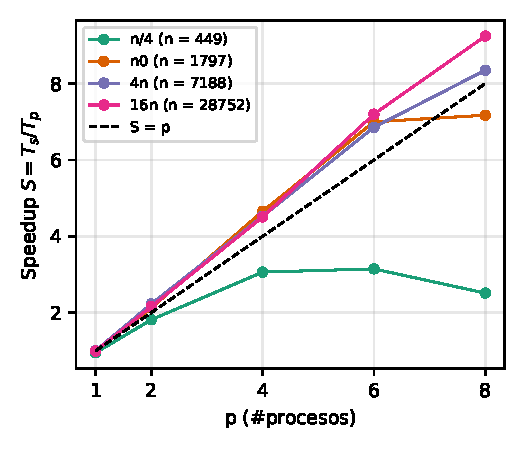
\includegraphics[width=0.45\textwidth]{figuras/F4_speedup.pdf}\hfill
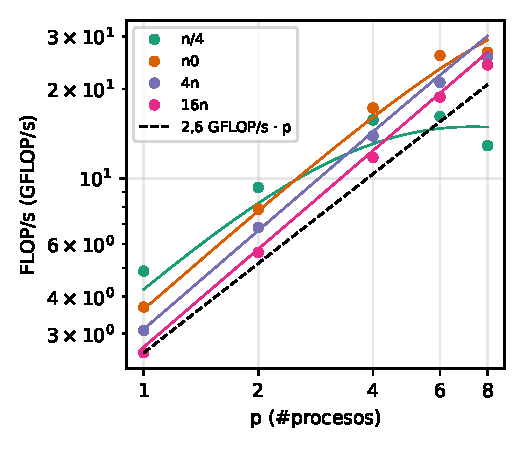
\includegraphics[width=0.45\textwidth]{figuras/F5_flops.pdf}
\caption{Izquierda: \textit{speedup} $S = T_s/T_p$. Derecha: velocidad en FLOP/s (marcadores), la curva teórica $\text{FLOP}_{total}/T_p^{teo}$ (líneas) y la recta ideal. Fuente: elaboración propia.}
\label{fig:speedup}
\end{figure}

La velocidad en FLOP/s (Figura~\ref{fig:speedup}, derecha) va de 2,6--4,9 GFLOP/s con un proceso a 24--27 GFLOP/s con 8 procesos (salvo $n/4$, que llega a 16,1 GFLOP/s con $p = 6$ y baja a 12,9 con $p = 8$). Como el número de FLOP es el mismo en paralelo y en secuencial, $\text{FLOPs}(p)/\text{FLOPs}_{sec} = T_s/T_p = S$: la gráfica de FLOP/s es el \textit{speedup} multiplicado por la velocidad secuencial, pero muestra además el valor absoluto. Para $n/4$ la curva teórica se aplana cerca de $p \approx 7$ (unos 15 GFLOP/s, sin bajar con $p = 8$), pero la velocidad medida cae un 20\,\% de $p = 6$ a 8: el modelo no capta esa caída.

\subsection{Escalabilidad}
\label{sec:esc}

Siguiendo el curso [8], la función de \textit{overhead} es $T_0 = p\,T_p - W$, con $W = \ntr\nte = 0{,}16\,n^2$ y todo en función de un solo $n$:
\[
T_0 = O\big(n\, k\, p^2 (1 + b) + a\,p\log p + b\,n\,p\,(1 + \log p)\big),
\qquad E = \frac{1}{1 + T_0/W}.
\]
Aquí contamos $W$ en pares ($\ntr\nte$) y no en operaciones como en la Sección~\ref{sec:pram}; como cada par cuesta $O(d) = O(1)$, las dos cuentas son $\Theta(n^2)$ y el análisis no cambia. $W$ no incluye el ordenamiento (suponemos $d > \log_2\ntr$). En la beta 3 cada proceso ordena listas de $\ntr/p$, así que $p\,T_{comp_1}$ es menor que $T_s$; por eso medimos $E > 1$. Si $W$ incluyera el ordenamiento, $T_0$ ganaría el término negativo $-c_s\,\ntr\nte\log_2 p$ (cada proceso ordena listas $p$ veces más cortas), que es el que da $E > 1$; cuando $T_0 < 0$, como en $4n$ y $16n$, $W = K\,T_0$ no tendría solución con $K > 0$. Por eso tomamos como $W$ el costo del mejor secuencial, $\Theta(n^2)$ sin ordenar, y con ese $W$ valen las condiciones de la Tabla~\ref{tab:iso}.
Para mantener $E$ constante se necesita $W = K\cdot T_0$, con $K = E/(1-E)$ [8] (en mayúscula para no confundirla con los $k$ vecinos), término a término (Tabla~\ref{tab:iso}). Por la regla del máximo, la condición que manda es
\[
n = \Theta(k\,p^2), \qquad\text{es decir}\qquad W = \Theta(k^2 p^4):
\]
si $p$ se duplica, $n$ debe crecer 4 veces y el trabajo 16 veces. Con la división 80/20 fija, $\ntr$ y $\nte$ crecen juntos; si se pudiera cambiar esa proporción, bastaría $\nte = \Theta(p)$ y $\ntr = \Theta(k\,p^2)$, o sea $W = \Theta(k\,p^3)$, que es menos exigente.

\begin{table}[!htb]
\centering
\small
\begin{tabular}{lll}
\toprule
\textbf{Término de $T_0$} & \textbf{Origen} & \textbf{Condición para $W = K\,T_0$} \\
\midrule
$n\,k\,p^2(1+b)$ & gather de candidatos y mezcla en el maestro & $n = \Theta(k\,p^2)$ \\
$a\,p\log p$ & latencias de broadcast, scatter y gather & $n = \Theta(\sqrt{p\log p})$ \\
$b\,n\,p$ & datos del scatter & $n = \Theta(p)$ \\
$b\,n\,p\log p$ & datos del broadcast & $n = \Theta(p\log p)$ \\
\bottomrule
\end{tabular}
\caption{Condiciones de isoeficiencia, con un solo $n$ ($W = \Theta(n^2)$).}
\label{tab:iso}
\end{table}

Hicimos tres experimentos (Figuras~\ref{fig:eficiencia} y \ref{fig:escalabilidad}, Tabla~\ref{tab:esc}). El primero mira la escalabilidad fuerte, que es el punto de vista de Amdahl ($n$ fijo), y los otros dos hacen crecer el problema con $p$, que es el punto de vista de Gustafson [5]:
\begin{itemize}[nosep]
  \item \textbf{E. Fuerte ($n$ constante):} con $n$ fijo el denominador de $E$ crece como $k\,p^2 + p\log p + p$, así que el algoritmo \textbf{no es escalable} con $n$ fijo. Se ve claramente en $n/4$ ($E = 0{,}31$ con $p = 8$) y en $n_0$ ($E$ baja de 1,17 a 0,90 entre $p = 6$ y $p = 8$). Para $4n$ y $16n$, $E$ se mantiene sobre 1 en $2 \le p \le 8$ (solo baja un poco entre $p = 6$ y $8$) porque $T_0/W$ es muy pequeño.
  \item \textbf{E. Débil (Gustafson, $n \propto \sqrt{p}$):} si $n$ crece como $\sqrt{p}$, el trabajo por proceso queda constante ($W/p = 0{,}16\,n^2/p \approx 517\,320$ pares en los cuatro puntos). La eficiencia débil $E_w = T(1)/T(p)$ da 1,06 y 1,08 con $p = 2$ y $4$, y baja a 0,83 con $p = 8$. Eso es lo que predice la teoría: con $n \propto \sqrt{p}$ el \textit{overhead} relativo $k\,p^2/n$ crece como $p^{1{,}5}$, así que esta ley no mantiene $E$ constante. Con $p \le 4$ la caída todavía no se ve porque las listas que ordena cada proceso se acortan ($\ntr/p$ baja de 1437 a 719 y $\log_2(\ntr/p)$ de 10,5 a 9,5). Con $p = 8$ se suma el hardware compartido: en las 4 repeticiones de ese punto, algún proceso perdió entre 8 y 18\,\% de su tiempo de CPU frente a otros programas (Sección~\ref{sec:dif}).
  \item \textbf{Isoeficiencia ($n \propto k\,p^2$):} de $n_0 = 1797$ a 115\,008 imágenes, o sea 2\,119 millones de pares con $p = 8$. La eficiencia se mantiene casi plana ($E = 0{,}99$, 1,11, 1,13 y 1,13 para $p = 1, 2, 4, 8$), que es justo lo que predice la condición $n = \Theta(k\,p^2)$. Con $p \le 8$ esto es consistente con la teoría pero no la prueba: el \textit{overhead} todavía es mucho menor que el cómputo, y el $E$ un poco mayor que 1 viene del ordenamiento (Sección~\ref{sec:dif}).
\end{itemize}

\begin{figure}[!htb]
\centering
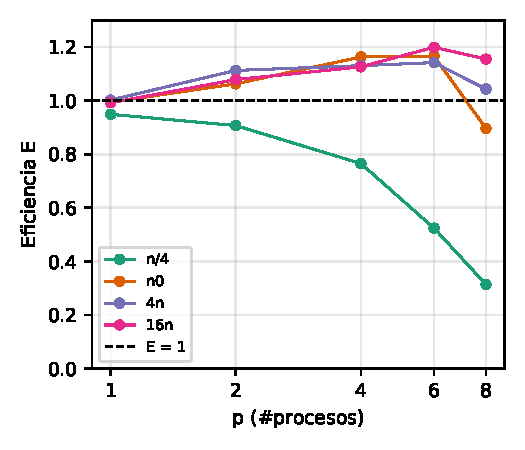
\includegraphics[width=0.45\textwidth]{figuras/F6_eficiencia.pdf}
\caption{Eficiencia $E = T_s/(p\,T_p)$ con $n$ fijo, para cada tamaño. Fuente: elaboración propia.}
\label{fig:eficiencia}
\end{figure}

\begin{figure}[!htb]
\centering
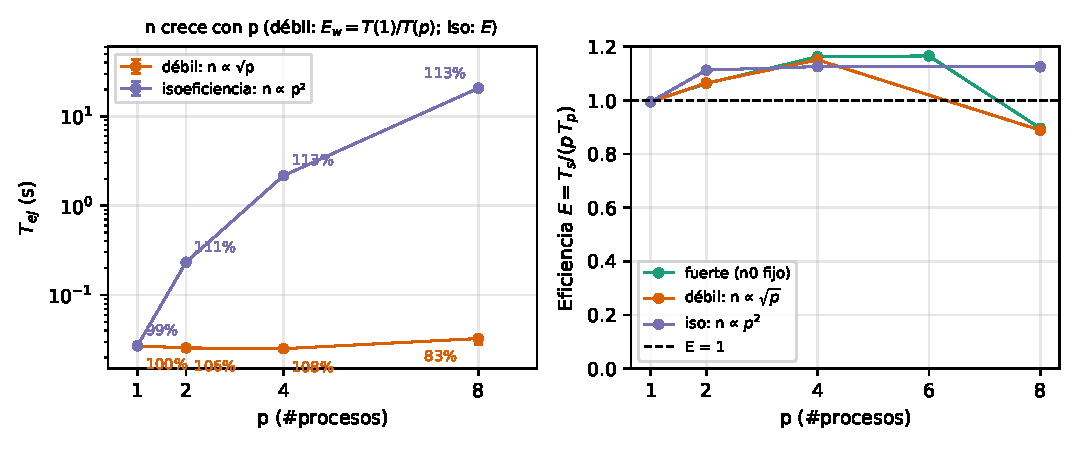
\includegraphics[width=0.92\textwidth]{figuras/F7_escalabilidad.pdf}
\caption{Izquierda: tiempo cuando $n$ crece con $p$ (en \% la eficiencia débil $E_w$ para la serie débil y $E$ para la de isoeficiencia). Derecha: eficiencia de los tres experimentos. Fuente: elaboración propia.}
\label{fig:escalabilidad}
\end{figure}

\begin{table}[!htb]
\centering
\small
\begin{tabular}{lrrrrrcc}
\toprule
\textbf{Experimento} & $p$ & $\mathbf{n}$ & $\mathbf{\ntr}$ & $T_{ej}$ (ms) & $T_s$ (ms) & $E$ & $E_w$ \\
\midrule
débil ($n \propto \sqrt{p}$) & 1 & 1\,797 & 1\,437 & 27,0 & 26,8 & 0,99 & 1,00 \\
débil ($n \propto \sqrt{p}$) & 2 & 2\,541 & 2\,032 & 25,5 & 54,4 & 1,06 & 1,06 \\
débil ($n \propto \sqrt{p}$) & 4 & 3\,594 & 2\,874 & 25,0 & 115,3 & 1,15 & 1,08 \\
débil ($n \propto \sqrt{p}$) & 8 & 5\,082 & 4\,064 & 32,5 & 231,5 & 0,89 & 0,83 \\
iso ($n \propto p^2$) & 1 & 1\,797 & 1\,437 & 27,0 & 26,8 & 0,99 & -- \\
iso ($n \propto p^2$) & 2 & 7\,188 & 5\,748 & 232,8 & 518,0 & 1,11 & -- \\
iso ($n \propto p^2$) & 4 & 28\,752 & 22\,992 & 2165,6 & 9754,9 & 1,13 & -- \\
iso ($n \propto p^2$) & 8 & 115\,008 & 91\,968 & 20633,2 & 185718,4 & 1,13 & -- \\
\bottomrule
\end{tabular}
\caption{Escalabilidad débil e isoeficiencia, con un solo $n$ ($\ntr = 0{,}8n$, $\nte = 0{,}2n$): mediana de 4 repeticiones (2 con 115\,008 imágenes). La fila con $p = 1$ es la misma medición en las dos series.}
\label{tab:esc}
\end{table}

\subsection{Diferencias entre la teoría y el experimento}
\label{sec:dif}

\begin{itemize}[nosep]
  \item \textbf{Constantes ocultas:} en la beta 3 el ordenamiento pesa más que las distancias, al revés de lo que supusimos con $d = 64$ en la entrega parcial. Esto da el \textit{speedup} superlineal.
  \item \textbf{Hardware compartido:} en una prueba aparte (\texttt{pruebas\_extra.py}) corrimos 8 copias independientes del mismo cálculo y cada una tardó 29,8 ms en promedio (31,4 ms la más lenta) frente a 26,6 ms sola (1,12 veces más; 1,02 con 4 copias). El mismo efecto se ve en la serie de control con $\nte$ fijo y $\ntr \propto p$ (así $\ntr/p = 1437$ no cambia y el ordenamiento cuesta lo mismo): el cómputo local sube de 26,2 a 32,4 ms con $p = 8$, un 24\,\% más. Con $p = 8$ los 8 núcleos de rendimiento están ocupados, así que cualquier otro programa le quita CPU a algún proceso o lo hace correr en un núcleo de eficiencia; además, los procesos comparten memoria y frecuencia. Eso explica la caída de $E_w$ con $p = 8$ en la serie débil, y que el modelo, que no incluye nada de esto, subestime el tiempo con $p = 8$ en $4n$ (52,8 frente a 62,1 ms) y en la isoeficiencia (17,6 frente a 20,6 s).
  \item \textbf{Serialización:} las colectivas en minúscula usan \textit{pickle}. En el ping-pong, la latencia con objetos es 10 veces la de los búferes (5,3 frente a 0,5 $\mu$s) y el costo por dato 4,6 veces (2,0 frente a 0,43 ns).
  \item \textbf{Parte secuencial en el maestro:} la mezcla de los $p\cdot k$ candidatos crece con $p$ y para $n/4$ ya es comparable al cómputo.
  \item \textbf{Desbalance:} como $\ntr$ puede no ser múltiplo de $p$ (por ejemplo, 1437), los bloques difieren en una fila; el desbalance medido es de 0--9\,\%, salvo $n_0$ con $p = 8$ (22\,\%) y $n/4$ con $p = 6$ y $8$ (26 y 84\,\%), donde el cómputo por proceso dura menos de 3,5 ms y cualquier interrupción del sistema pesa más.
\end{itemize}

\subsection{Mejoras}
\label{sec:mejoras}

\begin{itemize}[nosep]
  \item \textbf{Seleccionar en vez de ordenar:} usar \texttt{np.argpartition} para los $k$ menores ($O(\ntr/p)$ en lugar de $O(\ntr/p\,\log(\ntr/p))$). Como el ordenamiento domina, esto bajaría $T_{comp_1}$ y quitaría el \textit{speedup} superlineal.
  \item \textbf{Reducción en árbol en vez de gather (beta 3b, implementada):} mezclamos los candidatos de dos en dos con \texttt{comm.reduce} y un operador que deja los $k$ menores. En teoría, el término $n\,k\,p$ pasa a $n\,k\log p$ y la condición de isoeficiencia baja de $n = \Theta(k\,p^2)$ a $n = \Theta(k\,p\log p)$ [5], [8]. Con $p = 8$, el tiempo de los pasos 5 a 7 baja un 33\,\% en $16n$ (de 6,9 a 4,6 ms), pero ahí esos pasos son menos del 1\,\% de $T_{ej}$; en $n_0$ y $4n$ casi no cambia (2\,\%). El tiempo total cambia a lo más un 4\,\% en $n_0$, $4n$ y $16n$, del orden del ruido; en $n/4$, donde una corrida dura alrededor de 1 ms, la 3b es hasta 9\,\% más lenta (Figura~\ref{fig:reduccion}). Como anticipó el profesor, el ahorro es pequeño [10]: con $p \le 8$ el gather todavía no es un cuello de botella.
  \item \textbf{Colectivas con búfer:} \texttt{Bcast}, \texttt{Scatterv} y \texttt{Gatherv} sobre arreglos de NumPy evitan \textit{pickle}: en el ping-pong, la latencia baja de 5,3 a 0,5 $\mu$s y el costo por dato de 2,0 a 0,43 ns.
  \item \textbf{Evitar el scatter:} si cada proceso lee su propio bloque de entrenamiento, se elimina el término $b\,\ntr$, como en el algoritmo optimizado de la PD02 (Algorithm 6), que evita el scatter y el gather [6].
  \item \textbf{Paralelismo híbrido:} MPI entre nodos e hilos dentro de cada nodo aumenta la granularidad, aunque no necesariamente es más eficiente [7].
\end{itemize}

\begin{figure}[!htb]
\centering
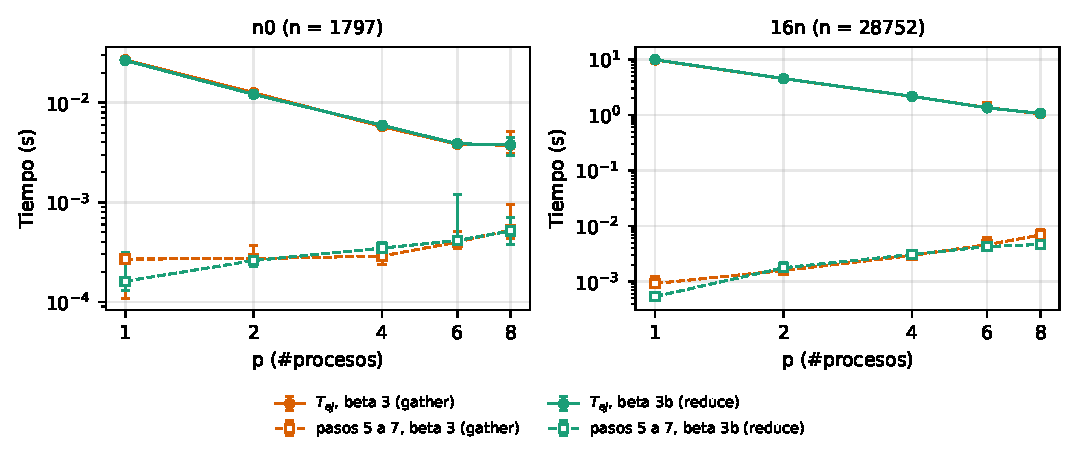
\includegraphics[width=0.92\textwidth]{figuras/F11_gather_vs_reduccion.pdf}
\caption{Beta 3 (gather) frente a beta 3b (reducción en árbol) con $n_0$ y $16n$: tiempo de ejecución y tiempo de los pasos 5 a 7. Fuente: elaboración propia.}
\label{fig:reduccion}
\end{figure}

\subsection{Síntesis}

El KNN en paralelo con bcast, scatter y gather mantiene exactamente las predicciones del código secuencial y es \textit{compute bound} para los tamaños que medimos, salvo el más pequeño. La expresión teórica de la entrega parcial, normalizada con constantes medidas por fase, reproduce los tiempos con un error medio de 8\,\%. El número óptimo de procesos crece como $\sqrt{n}$ (unos 18 para $n = 1797$) y el algoritmo solo escala si $n$ crece como $k\,p^2$. La reducción en árbol da las mismas predicciones, con un ahorro pequeño.

%====================================================================
\section{Bibliografía}

\begin{enumerate}[label={[\arabic*]}, leftmargin=*, itemsep=3pt]
  \item J. Fiestas, \textit{Computación Paralela y Distribuida: Proyecto -- Laboratorio}, 2026-II. Lima, Perú: UTEC, 2026.\\
  \textbf{Impacto:} define el caso 5, el DAG (Figura~\ref{fig:dag}) y lo que debe tener el informe final.

  \item \texttt{knn\_digits\_sec.py}, código secuencial del caso 5, adjunto al enunciado del proyecto [1]. [Online]. Available: \url{https://drive.google.com/file/d/1wTBSh7bwT1QVvce0pFMv5tcCWsg4-HeK/view} (accessed Sep. 18, 2026).\\
  \textbf{Impacto:} es el código que paralelizamos y la referencia para validar las predicciones y la precisión.

  \item L. Dalcin, \textit{MPI for Python (mpi4py) documentation} [Online]. Available: \url{https://mpi4py.readthedocs.io/en/stable/} (accessed Sep. 18, 2026).\\
  \textbf{Impacto:} uso de \texttt{comm.bcast}, \texttt{comm.scatter}, \texttt{comm.gather}, \texttt{comm.Barrier} y \texttt{MPI.Wtime} en el código.

  \item F. Pedregosa \textit{et al.}, ``Scikit-learn: Machine Learning in Python,'' \textit{Journal of Machine Learning Research}, vol. 12, pp. 2825--2830, 2011.\\
  \textbf{Impacto:} librería de los datos (\texttt{load\_digits}) y del \textit{split} del código base.

  \item J. Fiestas, diapositivas y apuntes del curso CS4052 (2026-II): U1.2 Foster y Flynn, U1.3 DAG, U2.1 Performance, U2.2 y U2.3 PRAM, U2.4 Particionamiento. Lima, Perú: UTEC, 2026.\\
  \textbf{Impacto:} base teórica del PRAM, de $S$ y $E$, del modelo $T_{comm} = f(p)(\alpha + x\beta)$, de la granularidad $G = T_{comp}/T_{comm}$ y de la mejora con reducción en árbol.

  \item J. Fiestas, \textit{CS4052 -- Prácticas Dirigidas 01 y 02 (soluciones)}. Lima, Perú: UTEC, 2026.\\
  \textbf{Impacto:} modelo del pseudocódigo distribuido, de la forma $E = O(1/(1 + \dots))$ y de la mejora sin scatter.

  \item J. Fiestas, diapositivas del curso CS4052: U4.5 Paralelismo híbrido. Lima, Perú: UTEC, 2026.\\
  \textbf{Impacto:} usar un proceso MPI por núcleo físico y plantear el paralelismo híbrido como mejora.

  \item J. Fiestas, diapositivas del curso CS4052: U6.1 Performance--Broadcast y U6.2 Performance y escalabilidad, y código \texttt{knn.cpp} de la PD04 (material del semestre 2026-I). Lima, Perú: UTEC, 2026.\\
  \textbf{Impacto:} modelo $T(m) = \alpha + m\beta$ de las colectivas y reducción en árbol; conteo de FLOP y FLOP/s; versión secuencial considerada para $T_s$ y \textit{speedup} superlineal; función de \textit{overhead} $T_0$, isoeficiencia y regla del máximo; cálculo de $p_{opt}$ con $T'(p) = 0$; datos sintéticos para escalar el problema.

  \item Anthropic, \textit{Claude Opus 5} y \textit{Claude Opus 5.5} (asistentes de inteligencia artificial, usados con Claude Code), setiembre a noviembre de 2026.\\
  \textbf{Uso:} resumió el material del curso; escribió el código de las tres versiones beta, de la mejora con reducción y de los scripts de experimentos, ping-pong, validación y análisis; ejecutó las mediciones; y redactó el borrador de este informe y de la presentación.\\
  \textbf{Impacto y validación:} la mayor parte del código y del texto se hizo con esta herramienta. Validamos el código comparando las predicciones con las del código base del profesor para $p = 1$ a $8$ (Sección~\ref{sec:validacion}) y revisamos las fórmulas y el análisis con el material del curso [5]--[8]. Las cifras del análisis salen de los datos y scripts del .zip adjunto. El grupo es responsable del contenido presentado.

  \item J. Fiestas, respuesta por correo electrónico a una consulta del grupo sobre el costo de \texttt{scatter} y \texttt{gather} y el acceso al clúster Khipu, 6 de noviembre de 2026 (comunicación personal).\\
  \textbf{Impacto:} aclara que $O(p)$ es la aproximación no optimizada y que MPI usa $O(\log p)$, con la expresión de la U2.4 (Tabla~\ref{tab:pasos}); acepta la reducción en árbol como mejora (Sección~\ref{sec:mejoras}); y justifica medir en una computadora personal porque Khipu no estaba disponible (Sección~\ref{sec:experimental}).
\end{enumerate}

\end{document}
